%%%%%%%%%%%%%%%%%%%%%%%%%%%%%%%%%%%%%%%%%
%\title{Title page with logo}
%----------------------------------------------------------------------------------------
%	PACKAGES AND OTHER DOCUMENT CONFIGURATIONS
%----------------------------------------------------------------------------------------

\documentclass[12pt]{article}
\usepackage[english]{babel}
\usepackage[utf8x]{inputenc}
\usepackage{amsmath}
\usepackage{graphicx}
\usepackage[colorinlistoftodos]{todonotes}

\begin{document}

\begin{titlepage}

\newcommand{\HRule}{\rule{\linewidth}{0.5mm}} % Defines a new command for the horizontal lines, change thickness here

\center % Center everything on the page
 
%----------------------------------------------------------------------------------------
%	HEADING SECTIONS
%----------------------------------------------------------------------------------------

\textsc{\LARGE Università degli studi di Milano Bicocca}\\[1.5cm] % Name of your university/college
\textsc{\Large Gruppo-BrewDay-2}\\[0.5cm] % Major heading such as course name
\textsc{\large Progetto-BrewDay-2}\\[0.5cm] % Minor heading such as course title

%----------------------------------------------------------------------------------------
%	TITLE SECTION
%----------------------------------------------------------------------------------------

\HRule \\[0.4cm]
{ \huge \bfseries Brew Day!}\\[0.4cm] % Title of your document
\HRule \\[1.5cm]
 
%----------------------------------------------------------------------------------------
%	AUTHOR SECTION
%----------------------------------------------------------------------------------------

\begin{minipage}{0.45\textwidth}
\begin{flushleft} \large
\emph{Author:}\\
David \textsc{Chieregato} 806961 % Your name
Davide \textsc{Ditolve} 806953
\end{flushleft}
\end{minipage}
~
\begin{minipage}{0.45\textwidth}
\begin{flushright} \large
~\newline
Chunhua \textsc{He} 804350\\
Luca \textsc{De Filippi} 757401\\
\end{flushright}
\end{minipage}\\[2cm]

% If you don't want a supervisor, uncomment the two lines below and remove the section above
%\Large \emph{Author:}\\
%John \textsc{Smith}\\[3cm] % Your name
%----------------------------------------------------------------------------------------
%	LOGO SECTION
%----------------------------------------------------------------------------------------


\includegraphics{logo.jpg}\\[3cm] % Include a department/university logo - this will require the graphicx package
 
%----------------------------------------------------------------------------------------

\vfill % Fill the rest of the page with whitespace

\end{titlepage}


\begin{abstract}
Home brewing, the process of producing beer on a small scale for personal purposes, is an activity that receives growing attention among beer enthusiasts. Every home brewer owns a brewing equipment (kettles, fermenters, pipes, etc.) with a certain maximum brewing capacity, the number of litres the equipment is able to handle in a single "batch". Brewing also requires ingredients, whose actual amounts vary from recipe to recipe; these are various kinds of malts, hops, yeasts and sugars (and of course, water). Brewers like to log their recipes, for future reference, and maintain an updated list of available ingredients, for shopping before the next brew.

The goal of this project is to develop an application for home brewers thats allows them to maintain a list of recipes, and adapt existing ones. The application must also maintain a list of available ingredients, update this list after a batch and when new ingredients are bought, and produce shopping lists for the next batch. A special characteristic of the application is the "what should I brew today?" feature: it goes through the recipes, and taking into account the available ingredients and brewing capacity of the equipment selects a recipe that can be brewed with the available ingredients, maximizing the use of the ingredients, and the batch size.
Brew Day! is an application that allows home brewers to maintain an organized database of their beer recipes. The application allows users to create, store and modify recipes, and later on delete them, if the user wishes to do so. The application is intended for "all-grain" brewers only, and thus all recipes are for this kind of brews (the "extract" brews are not supported).

Every home brewer has a specific equipment, whose characteristics leads to a particular "batch size", the maximum number of litres that can be brewed on a single run. Recipes involve, besides water:
malts
hops
yeasts
sugars
additives
While brewers prefer to create recipes referring to concrete values, like kilograms of a specific malt or grams of a specific hops, the application must store these recipes in some "absolute" measure, that allows for a direct conversion of the recipe when the equipment, and consequently the batch size, is updated. For instance, expressing malt quantities as a percentage of the total, and hops as grams per litre of mash, is a possibility.

Besides the actual recipes, the application must maintain recipe instances, i.e., particular brews based on a recipe; these instances can be accompanied by notes to refer to issues that may affect the resulting beer and the brewers would like to keep logged. A particular kind of note is the tasting notes, that allows brewers to keep track of opinions on a beer from a particular brew.

Besides these more traditional features of Brew Day!, the application maintains a list of available ingredients. This allows brewers to be notified about missing ingredients for the next brew. A recipe instance, i.e., a particular brew, should allow users to update the available ingredients list, substracting used ingredients from the available ones. Related to this information, Brew Day! must support a useful feature for brewers: "what should I brew today?" goes through the recipes database, and chooses the recipe that maximizes the use of the available ingredients, taking into account the equipment capacity, of course.

The project must implement the features described above, i.e., creation, modification and deletion of recipes, creation of recipe instances (brews), support for notes on brews, and keeping track of available ingredients. The "what should I brew today?" is a mandatory feature. Optionally, developers may choose to allow ingredients availability manually, as opposed to do it automatically from brews information.

The choice of the development platform, including tools and programming languages to use, is left to the teams. The application may be desktop-based, web-based or even tailored for portable devices. Besides the development of the software, teams must provide accompanying documentation, including a requirements document, a design document, and a brief user manual (installation and usage of the application).

\end{abstract}
\section{Assunzioni e glossario}
\section{Requisiti}

The goal of this project is to develop an application for home brewers thats allows them to mantain a list of recipes, and adapt esisting ones.
This application is intended for the "all-grain" users only, thus "extract" brews are not supported. \\\
\\
\\
Functional Requirements:\\
\\
\\
User's account:

The application allows users to create an account

The application allows users to login in their account

	Every user have specific equipment which can produce a maximum "batch size"
\\
\\
User's recipe:
	
The application allows users to create a recipe

The application allows users to store a recipe 

The application allows users to update a recipe

The application allows users to delete a recipe

The application stores recipe's ingredients in an "absolute" measure; eg. total percentage

	Recipes are made by ingredients: Water, Malts, Hops, Yeasts, Sugars, Additives
\\
\\
Recipes ingredients:

The application mantain a list of available ingredients

The application notifies users about missing ingredients

The application update ingredients's list after a batch

The application update ingredients's list when new ingredients are bought

The application produce a shopping list for the next batch 
\\
\\
Additional features:

The application has "what should i brew today" feature.

	With the "what should i brew today" feature, the application suggest a recipe made with the available ingredients.

	With the "what should i brew today" feature, the suggested recipe maximizes the usage of available ingredients.

	With the "what should i brew today" feature, the suggested recipe maximizes the batch size.
	
The application supports notes for brews


\section{Casi d'uso}
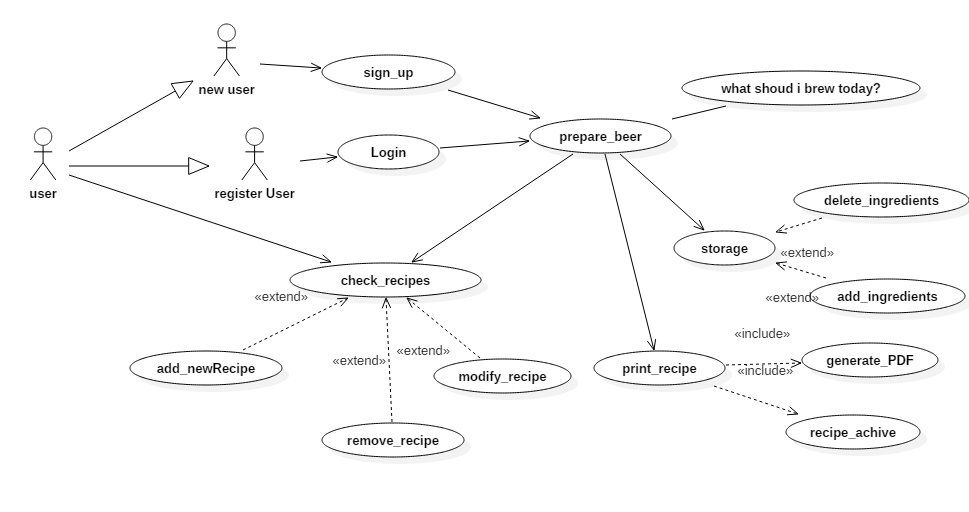
\includegraphics{UseCaseDiagram.png}\\
\label{cd:primo}

\subsection{Primo}
...\\
\todo[inline, color=green!40]{This is an inline comment.}

% Commands to include a figure:
\begin{figure}
\centering

\includegraphics[width=0.5\textwidth]{logo.jpg}
\caption{\label{fig:frog}This is a figure caption.}
\end{figure}

\begin{table}
\centering
\begin{tabular}{l|r}
Item & Quantity \\\hline
Widgets & 42 \\
Gadgets & 13
\end{tabular}
\caption{\label{tab:widgets}An example table.}
\end{table}

\subsection{Lists}

\begin{enumerate}
\item Like this,
\item and like this.
\end{enumerate}
\dots or bullet points \dots
\begin{itemize}
\item Like this,
\item and like this.
\end{itemize}

\section{Attività}

\section{Sequenza}

\section{Dominio}

\section{Componenti}

\section{Classi}

\section{Iterazione}

\section{Stato}

\section{Test}

\end{document}
